% ============================================================
%  Programación Científica 2026-1 — UNAL
%  Módulo: Diferenciación Automática
%  Clase única (90 min)
% ============================================================
\documentclass[aspectratio=169,10pt]{beamer}

% ---------- fuente sans-serif limpia ----------
\usepackage[T1]{fontenc}
\usepackage{helvet}
\renewcommand{\familydefault}{\sfdefault}

% ---------- paquetes ----------
\usepackage{amsmath,amssymb,bm}
\usepackage{tikz}
\usetikzlibrary{positioning,arrows.meta,calc,matrix,decorations.pathreplacing,shapes.geometric}
\usepackage{tcolorbox}
\tcbuselibrary{skins,breakable}
\usepackage{listings}
\usepackage{booktabs}
\usepackage{colortbl}
\usepackage{graphicx}
\usepackage{xcolor}

% ============================================================
%  PALETA DE COLORES
% ============================================================
\definecolor{darkbg}{HTML}{1C1C2E}
\definecolor{lightbg}{HTML}{F7F7F9}
\definecolor{accent}{HTML}{6C63FF}
\definecolor{accentteal}{HTML}{1DB89A}
\definecolor{accentamber}{HTML}{F4A623}
\definecolor{accentcoral}{HTML}{E05A4E}
\definecolor{textdark}{HTML}{1C1C2E}
\definecolor{textlight}{HTML}{F7F7F9}
\definecolor{textgray}{HTML}{6B6B80}
\definecolor{codefg}{HTML}{E8E8F0}
\definecolor{codebg}{HTML}{272740}

% ============================================================
%  TEMA BEAMER
% ============================================================
\setbeamertemplate{navigation symbols}{}
\setbeamertemplate{footline}{
  \begin{beamercolorbox}[wd=\paperwidth,ht=2.2ex,dp=1.2ex,rightskip=4mm]{footline}
    \hfill\usebeamerfont{footline}%
    \textcolor{textgray}{\tiny Programación Científica 2026-1 \quad|\quad
      Diferenciación Automática \quad|\quad \insertframenumber/\inserttotalframenumber}%
    \hspace{2mm}
  \end{beamercolorbox}
}

\setbeamercolor{normal text}{fg=textdark,bg=lightbg}
\setbeamercolor{frametitle}{fg=textdark,bg=lightbg}
\setbeamertemplate{frametitle}{
  \vspace{4pt}
  \begin{beamercolorbox}[wd=\textwidth,leftskip=2mm]{frametitle}
    \usebeamerfont{frametitle}\insertframetitle
    \ifx\insertframesubtitle\empty\else
      \par\vspace{1pt}
      {\footnotesize\textcolor{textgray}\insertframesubtitle}
    \fi
  \end{beamercolorbox}
  \vspace{-2pt}
  {\color{accent}\rule{\textwidth}{0.6pt}}
  \vspace{2pt}
}
\setbeamerfont{frametitle}{size=\large,series=\bfseries}

% ============================================================
%  CAJAS DE CONTENIDO
% ============================================================
\newtcolorbox{defbox}[1]{
  enhanced, title=#1,
  colback=accent!8, colframe=accent, coltitle=white,
  fonttitle=\bfseries\small, boxrule=0.6pt,
  attach boxed title to top left={yshift=-2mm,xshift=4mm},
  boxed title style={colback=accent,boxrule=0pt},
  left=4pt,right=4pt,top=6pt,bottom=4pt
}

\newtcolorbox{resultbox}[1]{
  enhanced, title=#1,
  colback=accentteal!8, colframe=accentteal, coltitle=white,
  fonttitle=\bfseries\small, boxrule=0.6pt,
  attach boxed title to top left={yshift=-2mm,xshift=4mm},
  boxed title style={colback=accentteal,boxrule=0pt},
  left=4pt,right=4pt,top=6pt,bottom=4pt
}

\newtcolorbox{obsbox}[1]{
  enhanced, title=#1,
  colback=accentamber!10, colframe=accentamber, coltitle=white,
  fonttitle=\bfseries\small, boxrule=0.6pt,
  attach boxed title to top left={yshift=-2mm,xshift=4mm},
  boxed title style={colback=accentamber,boxrule=0pt},
  left=4pt,right=4pt,top=6pt,bottom=4pt
}

\newtcolorbox{taskbox}[1]{
  enhanced, title=#1,
  colback=accentcoral!8, colframe=accentcoral, coltitle=white,
  fonttitle=\bfseries\small, boxrule=0.6pt,
  attach boxed title to top left={yshift=-2mm,xshift=4mm},
  boxed title style={colback=accentcoral,boxrule=0pt},
  left=4pt,right=4pt,top=6pt,bottom=4pt
}

% ============================================================
%  CÓDIGO
% ============================================================
\lstset{
  language=Python,
  basicstyle=\ttfamily\scriptsize\color{codefg},
  backgroundcolor=\color{codebg},
  keywordstyle=\color{accent!80!white}\bfseries,
  stringstyle=\color{accentteal},
  commentstyle=\color{textgray}\itshape,
  numbers=none,
  frame=none,
  breaklines=true,
  xleftmargin=4pt, xrightmargin=4pt,
  aboveskip=4pt, belowskip=4pt,
  showstringspaces=false,
  morekeywords={jnp,jax,np,fft,ifft,grad}
}

% ============================================================
%  SLIDE OSCURO
% ============================================================
\newcommand{\darkslide}[1]{
  {
  \setbeamercolor{background canvas}{bg=darkbg}
  \setbeamertemplate{footline}{}
  #1
  }
}

% ============================================================
%  MACROS MATEMÁTICOS
% ============================================================
\newcommand{\R}{\mathbb{R}}
\newcommand{\C}{\mathbb{C}}
\newcommand{\norm}[1]{\left\|#1\right\|}
\newcommand{\adj}{{}^{H}}

% ============================================================
%  ESTILOS TIKZ PARA GRAFOS
% ============================================================
\tikzset{
  vnode/.style={
    circle, draw=accent, fill=accent!12,
    minimum size=22pt, font=\small, line width=0.5pt
  },
  outnode/.style={
    circle, draw=accentcoral, fill=accentcoral!15,
    minimum size=22pt, font=\small, line width=0.5pt
  },
  innode/.style={
    circle, draw=accentteal, fill=accentteal!15,
    minimum size=22pt, font=\small, line width=0.5pt
  },
  arr/.style={
    -{Stealth[length=4pt]}, line width=0.5pt, accent!70
  },
  arrback/.style={
    -{Stealth[length=4pt]}, line width=0.7pt, accentcoral, dashed
  },
  oplabel/.style={
    font=\tiny\itshape, color=textgray
  }
}

% ============================================================
%  PORTADA
% ============================================================
\title{\textbf{Diferenciación Automática}}
\subtitle{Módulo 3}
\author{Programación Científica 2026-1}
\institute{Universidad Nacional de Colombia}
\date{}

% ============================================================
\begin{document}
% ============================================================

% ---------- PORTADA ----------
\darkslide{
\begin{frame}[plain]
  \begin{tikzpicture}[remember picture, overlay]
    \fill[accent,opacity=0.15] (current page.north east) ++(-1,-1) circle (3.5cm);
    \fill[accentteal,opacity=0.10] (current page.south west) ++(2,2) circle (2.8cm);
    \fill[accentamber,opacity=0.08] (current page.south east) ++(-3,3) circle (1.8cm);
  \end{tikzpicture}
  \vspace{1.5cm}
  \begin{center}
    {\small\textcolor{accentteal}{\texttt{Programación Científica · UNAL · 2026-1}}}\\[10pt]
    {\LARGE\bfseries\textcolor{textlight}{Diferenciación Automática}}\\[6pt]
    {\large\textcolor{accent}{Módulo 3}}\\[18pt]
    {\small\textcolor{textgray}{El grafo computacional · JAX}}
  \end{center}
\end{frame}
}

% ============================================================
%  PARTE 1: MOTIVACIÓN
% ============================================================
\darkslide{
\begin{frame}[plain]
  \begin{tikzpicture}[remember picture, overlay]
    \fill[accentteal,opacity=0.12] (current page.north west) ++(1,-1) circle (2.5cm);
    \fill[accent,opacity=0.10] (current page.south east) ++(-2,1.5) circle (2cm);
  \end{tikzpicture}
  \vspace{2.2cm}
  \begin{center}
    {\LARGE\bfseries\textcolor{textlight}{¿Cómo derivamos una función dada como código?}}
  \end{center}
\end{frame}
}

% ----------
\begin{frame}{El problema}
\vspace{6pt}
Tenemos una función definida como código:
\[
\mathcal{L}(x) = (x^2 + 3x)\,\sin(x)
\]

\vspace{4pt}
Queremos $\dfrac{d\mathcal{L}}{dx}$ en algún punto $x_0$ específico.

\vspace{10pt}
\begin{defbox}{Pregunta}
¿Cómo lo calcula un computador, sin que nosotros derivemos a mano?
\end{defbox}

\vspace{8pt}
\textcolor{textgray}{Hay tres caminos...}
\end{frame}

% ----------
\begin{frame}{Opción 1: diferencias finitas}
\vspace{6pt}
Aproximar por definición de la derivada:
\[
\frac{d\mathcal{L}}{dx}(x_0) \;\approx\; \frac{\mathcal{L}(x_0 + h) - \mathcal{L}(x_0)}{h}
\]

\vspace{8pt}
\textbf{Ventajas:}
\begin{itemize}\small
  \item Trivial de implementar: solo evaluamos $\mathcal{L}$ dos veces.
  \item Funciona con \textbf{cualquier} código.
\end{itemize}

\vspace{6pt}
\textbf{Problemas:}
\begin{itemize}\small
  \item Error de truncamiento $O(h)$: si $h$ es grande, la aproximación es mala.
  \item Error de cancelación: si $h$ es muy pequeño, $\mathcal{L}(x_0+h) - \mathcal{L}(x_0)$ pierde dígitos significativos.
 % \item Para $n$ variables: \textbf{$n$ evaluaciones} de $\mathcal{L}$ (una por dimensión).
\end{itemize}
\end{frame}

% ----------
\begin{frame}{Opción 2: diferenciación simbólica}
\vspace{6pt}
Derivar la fórmula a mano (o con SymPy):
\[
\frac{d\mathcal{L}}{dx} = (2x+3)\sin(x) + (x^2+3x)\cos(x)
\]

\vspace{8pt}
\textbf{Ventajas:}
\begin{itemize}\small
  \item Resultado exacto (sin error numérico).
\end{itemize}

\vspace{6pt}
\textbf{Problemas:}
\begin{itemize}\small
  \item Hay que tener la \textbf{fórmula}: no sirve si $\mathcal{L}$ es un programa con condicionales, bucles, llamadas a funciones externas.
  \item \textbf{Expression swell}: derivar funciones compuestas produce expresiones que crecen explosivamente.
  \item Hay que re-derivar para cada nueva $\mathcal{L}$.
\end{itemize}

\vspace{6pt}
\textcolor{textgray}{\small Ejemplo de swell: la derivada de $f(f(f(x)))$ con la regla de la cadena triplica el tamaño.}
\end{frame}

% ----------
\begin{frame}{Opción 3: diferenciación automática (autodiff)}
\vspace{8pt}
\begin{defbox}{Idea}
Aplicar la regla de la cadena \textbf{paso a paso sobre el código}, descomponiendo $\mathcal{L}$ en operaciones elementales cuyas derivadas conocemos.
\end{defbox}

\vspace{10pt}
\textbf{Promesa:}
\begin{itemize}\small
  \item Exacto como la simbólica (sin error de truncamiento).
  \item Costo $O(1)$ evaluaciones de $\mathcal{L}$, sin importar el número de variables.
  \item Funciona con cualquier programa, no se necesita la fórmula.
\end{itemize}

\vspace{10pt}
\begin{obsbox}{Pregunta}
¿Cómo puede ser simultáneamente exacto, barato y general?\\
La respuesta está en el \textbf{grafo computacional}.
\end{obsbox}
\end{frame}


% ============================================================
%  PARTE 2: EL GRAFO COMPUTACIONAL
% ============================================================
\darkslide{
\begin{frame}[plain]
  
\begin{tikzpicture}[remember picture, overlay]
    \fill[accent,opacity=0.12] (current page.north east) ++(-1.5,-1) circle (3cm);
    \fill[accentteal,opacity=0.08] (current page.south west) ++(1.5,1) circle (2.2cm);
  \end{tikzpicture}
  \vspace{2.2cm}
  \begin{center}
    {\LARGE\bfseries\textcolor{textlight}{El grafo computacional}}
  \end{center}
\end{frame}
}

% ----------
\begin{frame}{Descomponer en operaciones elementales}
\vspace{6pt}
Función:
\[
\mathcal{L}(x) = (x^2 + 3x)\,\sin(x)
\]

\vspace{6pt}
Reescribirla introduciendo \textbf{variables intermedias} $v_i$, una por cada operación elemental:

\vspace{6pt}
\begin{center}
\begin{tabular}{ll}
\toprule
\textbf{Variable} & \textbf{Operación} \\
\midrule
$v_1 = x$           & entrada \\
$v_2 = v_1^2$       & potencia \\
$v_3 = 3\,v_1$      & escalar \\
$v_4 = v_2 + v_3$   & suma \\
$v_5 = \sin(v_1)$   & seno \\
$v_6 = v_4 \cdot v_5$ & producto \\
$\mathcal{L} = v_6$ & salida \\
\bottomrule
\end{tabular}
\end{center}
\end{frame}

% ----------
\begin{frame}{El grafo}
\vspace{4pt}
Cada $v_i$ es un \textbf{nodo}. Cada dependencia $v_i \to v_j$ es una \textbf{arista}.

\vspace{8pt}
\begin{center}
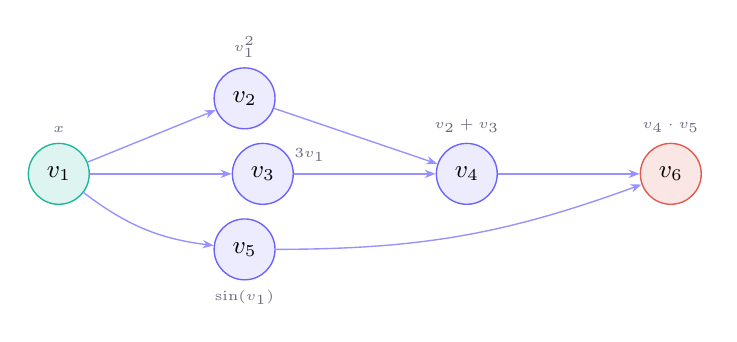
\begin{tikzpicture}[node distance=14mm and 14mm]
% nodos
\node[innode] (v1) {$v_1$};
\node[vnode, above right=4mm and 18mm of v1] (v2) {$v_2$};
\node[vnode, right=18mm of v1] (v3) {$v_3$};
\node[vnode, below right=4mm and 18mm of v1] (v5) {$v_5$};
\node[vnode, right=18mm of v3] (v4) {$v_4$};
\node[outnode, right=18mm of v4] (v6) {$v_6$};

% etiquetas
\node[oplabel, above=0pt of v1] {$x$};
\node[oplabel, above=0pt of v2] {$v_1^2$};
\node[oplabel, above right=-7pt and 0pt of v3] {$3v_1$};
\node[oplabel, below=0pt of v5] {$\sin(v_1)$};
\node[oplabel, above=0pt of v4] {$v_2+v_3$};
\node[oplabel, above=0pt of v6] {$v_4 \cdot v_5$};

% aristas
\draw[arr] (v1) -- (v2);
\draw[arr] (v1) -- (v3);
\draw[arr] (v1) to[bend right=15] (v5);
\draw[arr] (v2) -- (v4);
\draw[arr] (v3) -- (v4);
\draw[arr] (v4) -- (v6);
\draw[arr] (v5) to[bend right=10] (v6);
\end{tikzpicture}
\end{center}

%\begin{obsbox}{Observación}
%$v_1$ tiene \textbf{tres hijos}: $v_2$, $v_3$ y $v_5$. La regla de la cadena tendrá que sumar las contribuciones de los tres caminos por los que $x$ afecta a $\mathcal{L}$.
%\end{obsbox}
\end{frame}

% ----------
\begin{frame}{Propiedades del grafo}
\vspace{8pt}
\begin{itemize}
  \item \textbf{Dirigido}: cada arista tiene un sentido (de input hacia output).
  \item \textbf{Acíclico}: nunca regresa sobre sí mismo. 
  \item Los \textbf{nodos hoja} (sin padres) son los inputs.
  \item Los \textbf{nodos raíz} (sin hijos) son las salidas.
\end{itemize}

\vspace{10pt}
\begin{defbox}{Estrategia general}
Derivar $\mathcal{L}$ respecto a $x$ es \textbf{propagar derivadas} por las aristas, aplicando la regla de la cadena en cada nodo.
\end{defbox}

\vspace{6pt}
\textcolor{textgray}{Hay dos maneras de hacer esa propagación: hacia adelante (forward) o hacia atrás (reverse).}
\end{frame}

% ============================================================
%  PARTE 3: FORWARD MODE
% ============================================================
\darkslide{
\begin{frame}[plain]
  \begin{tikzpicture}[remember picture, overlay]
    \fill[accent,opacity=0.12] (current page.center) circle (3.5cm);
  \end{tikzpicture}
  \vspace{2.2cm}
  \begin{center}
    {\LARGE\bfseries\textcolor{textlight}{Forward mode: propagar tangentes}}
  \end{center}
\end{frame}
}

% ----------
\begin{frame}{Idea: arrastrar la derivada con cada valor}
\vspace{6pt}
Junto a cada $v_i$ propagamos su derivada respecto a la entrada:
\[
\dot{v}_i \;=\; \frac{\partial v_i}{\partial x}
\]

\vspace{6pt}
\textbf{Inicialización:} en la entrada, $\dot{v}_1 = \dot{x} = 1$.

\vspace{8pt}
\textbf{Propagación:} para cada nodo $v_j = g(v_i, \ldots)$, aplicamos la regla de la cadena:
\[
\dot{v}_j \;=\; \sum_{i \in \text{padres}(j)} \frac{\partial v_j}{\partial v_i}\,\dot{v}_i
\]

\vspace{10pt}
\begin{resultbox}{Pasada forward}
Recorremos el grafo \textbf{en el orden natural} (de entradas a salida), calculando $v_i$ y $\dot{v}_i$ al mismo tiempo en cada nodo.
\end{resultbox}
\end{frame}

% ----------
\begin{frame}{Forward mode sobre $\mathcal{L}(x) = (x^2+3x)\sin(x)$}
\vspace{4pt}
Evaluamos en $x = 2$. Inicializamos $\dot{v}_1 = 1$.

\vspace{6pt}
\begin{center}
\begin{tabular}{lll l}
\toprule
\textbf{Nodo} & \textbf{Valor} $v_i$ & \textbf{Tangente} $\dot{v}_i$ & \textbf{Regla} \\
\midrule
$v_1 = x$           & $2$            & $1$ & entrada \\
$v_2 = v_1^2$       & $4$            & $2 v_1 \cdot \dot{v}_1 = 4$ & cadena \\
$v_3 = 3 v_1$       & $6$            & $3 \cdot \dot{v}_1 = 3$ & cadena \\
$v_4 = v_2 + v_3$   & $10$           & $\dot{v}_2 + \dot{v}_3 = 7$ & suma \\
$v_5 = \sin(v_1)$   & $\sin 2 \approx 0.909$ & $\cos(v_1)\cdot \dot{v}_1 = \cos 2 \approx -0.416$ & cadena \\
$v_6 = v_4 \cdot v_5$ & $\approx 9.093$ & $\dot{v}_4 v_5 + v_4 \dot{v}_5 \approx 2.205$ & producto \\
$\mathcal{L} = v_6$ & $\approx 9.093$ & $\dot{v}_6 \approx 2.205$ & salida \\
\bottomrule
\end{tabular}
\end{center}

\end{frame}

% ----------
\begin{frame}{Costo del forward mode}
\vspace{8pt}
\textbf{Una pasada forward} produce $\dfrac{\partial \mathcal{L}}{\partial x}$ para \textbf{una} entrada $x$.

\vspace{8pt}
Si $\mathcal{L}: \R^n \to \R$ (muchas entradas, una salida):

\vspace{8pt}
\begin{itemize}
  \item Necesitamos $n$ pasadas forward (una por cada $\partial \mathcal{L}/\partial x_i$). \vspace{8pt}
  \item Costo total: $O(n)$ veces el costo de evaluar $\mathcal{L}$.
\end{itemize}

\end{frame}

% ============================================================
%  PARTE 4: REVERSE MODE
% ============================================================
\darkslide{
\begin{frame}[plain]
  \begin{tikzpicture}[remember picture, overlay]
    \fill[accentteal,opacity=0.12] (current page.north east) ++(-1.5,-1) circle (3cm);
    \fill[accentcoral,opacity=0.10] (current page.south west) ++(1.5,1.5) circle (2.5cm);
  \end{tikzpicture}
  \vspace{2.2cm}
  \begin{center}
    {\LARGE\bfseries\textcolor{textlight}{Reverse mode: propagar adjuntos}}
  \end{center}
\end{frame}
}

% ----------
\begin{frame}{Cambio de perspectiva}
\vspace{6pt}
En lugar de propagar $\dot{v}_i = \dfrac{\partial v_i}{\partial x}$ hacia adelante, propagamos:
\[
\bar{v}_i \;=\; \frac{\partial \mathcal{L}}{\partial v_i}
\]
hacia atrás (de la salida hacia las entradas). El símbolo $\bar{v}$ se llama \textbf{adjunto} de $v$.

\vspace{8pt}
\begin{defbox}{Regla de acumulación}
Para cada nodo $v_i$ con hijos $v_j$:
\[
\bar{v}_i \;=\; \sum_{j \in \text{hijos}(i)} \bar{v}_j \cdot \frac{\partial v_j}{\partial v_i}
\]
\end{defbox}


\end{frame}

% ----------
\begin{frame}{Pasada reverse: cómo se ejecuta}
\vspace{4pt}
\textbf{Paso 1 — Forward:} evaluar $v_i$ en todos los nodos y guardar.

\vspace{6pt}
\textbf{Paso 2 — Inicializar el adjunto de salida:}
\[
\bar{\mathcal{L}} = 1
\]

\vspace{6pt}
\textbf{Paso 3 — Backward:} recorrer el grafo \textbf{en orden inverso}, aplicando la regla de acumulación.

\vspace{10pt}
\begin{resultbox}{Resultado clave}
\textbf{Una sola pasada backward} produce $\bar{v}_i$ para \textbf{todos} los nodos del grafo.
\end{resultbox}

\vspace{4pt}
\textcolor{textgray}{Costo: dos veces el costo de evaluar $\mathcal{L}$, independiente de $n$.}
\end{frame}

% ----------
\begin{frame}{Reverse mode sobre $\mathcal{L}(x) = (x^2+3x)\sin(x)$}
\vspace{4pt}
Forward (en $x=2$) ya nos dio los $v_i$. Ahora, hacia atrás, con $\bar{v}_6 = 1$:

\vspace{4pt}
\begin{center}
\small
\begin{tabular}{ll l}
\toprule
\textbf{Adjunto} & \textbf{Cálculo} & \textbf{Valor} \\
\midrule
$\bar{v}_6 = \bar{\mathcal{L}}$ & inicialización & $1$ \\
$\bar{v}_5 = \bar{v}_6 \cdot \dfrac{\partial v_6}{\partial v_5} = \bar{v}_6 \cdot v_4$ & producto & $1 \cdot 10 = 10$ \\
$\bar{v}_4 = \bar{v}_6 \cdot \dfrac{\partial v_6}{\partial v_4} = \bar{v}_6 \cdot v_5$ & producto & $1 \cdot 0.909 \approx 0.909$ \\
$\bar{v}_3 = \bar{v}_4 \cdot 1$ & suma & $\approx 0.909$ \\
$\bar{v}_2 = \bar{v}_4 \cdot 1$ & suma & $\approx 0.909$ \\
$\bar{v}_1 = \bar{v}_2 \cdot 2 v_1 + \bar{v}_3 \cdot 3 + \bar{v}_5 \cdot \cos(v_1)$ & tres hijos & $\approx 2.205$ \\
\bottomrule
\end{tabular}
\end{center}

\vspace{6pt}
\textbf{Resultado:} $\dfrac{d\mathcal{L}}{dx}\bigg|_{x=2} = \bar{v}_1 \approx 2.205$. \quad \textcolor{accentteal}{Coincide con forward y con el cálculo analítico.}
\end{frame}

% ----------
\begin{frame}{El paso clave: $v_1$ tiene tres hijos}
\[
\bar{v}_1 \;=\; \underbrace{\bar{v}_2 \cdot 2 v_1}_{\text{vía } v_2} \;+\; \underbrace{\bar{v}_3 \cdot 3}_{\text{vía } v_3} \;+\; \underbrace{\bar{v}_5 \cdot \cos(v_1)}_{\text{vía } v_5}
\]

\vspace{8pt}
\begin{center}
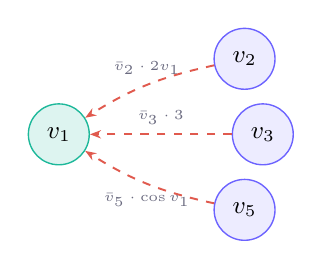
\begin{tikzpicture}[node distance=14mm and 14mm]
\node[innode] (v1) {$v_1$};
\node[vnode, above right=4mm and 18mm of v1] (v2) {$v_2$};
\node[vnode, right=18mm of v1] (v3) {$v_3$};
\node[vnode, below right=4mm and 18mm of v1] (v5) {$v_5$};

\draw[arrback] (v2) to[bend right=10] node[oplabel,above]{$\bar{v}_2 \cdot 2v_1$} (v1);
\draw[arrback] (v3) -- node[oplabel,above]{$\bar{v}_3 \cdot 3$} (v1);
\draw[arrback] (v5) to[bend left=10] node[oplabel,below]{$\bar{v}_5 \cdot \cos v_1$} (v1);
\end{tikzpicture}
\end{center}

\vspace{6pt}
\begin{resultbox}{Esto es la regla de la cadena multivariada}
Cada camino contribuye su propia derivada. Reverse mode \textbf{automatiza la suma}.
\end{resultbox}
\end{frame}

% ----------
\begin{frame}{Forward vs.\ reverse: cuándo usar cada uno}
\vspace{6pt}
\begin{center}
\begin{tabular}{lll}
\toprule
\textbf{Modo} & \textbf{Eficiente cuando} & \textbf{Costo} \\
\midrule
Forward  & pocas entradas, muchas salidas & $O(n)$ pasadas \\
\rowcolor{accentteal!12}
\textbf{Reverse} & \textbf{muchas entradas, una salida} & $O(1)$ pasadas \\
\bottomrule
\end{tabular}
\end{center}

\vspace{12pt}
\begin{defbox}{Reverse mode = backpropagation}
Cuando $\mathcal{L}$ es una función  escalar y $x$ son los parámetros, reverse mode es \textbf{el} algoritmo que hace posible las derivadas.
\end{defbox}

\vspace{8pt}
\textcolor{textgray}{En la práctica, autodiff casi siempre se refiere a reverse mode. JAX, PyTorch, TensorFlow lo usan por defecto con \texttt{grad}.}
\end{frame}

% ============================================================
%  PARTE 5: AUTODIFF EN LA PRÁCTICA
% ============================================================
\darkslide{
\begin{frame}[plain]
  \begin{tikzpicture}[remember picture, overlay]
    \fill[accentamber,opacity=0.10] (current page.north west) ++(2,-1.5) circle (3cm);
    \fill[accent,opacity=0.10] (current page.south east) ++(-2,2) circle (2.5cm);
  \end{tikzpicture}
  \vspace{2.2cm}
  \begin{center}
    {\LARGE\bfseries\textcolor{textlight}{Autodiff en la práctica}}
  \end{center}
\end{frame}
}

% ----------
\begin{frame}[fragile]{\texttt{jax.grad} en una línea}
\vspace{4pt}
\begin{lstlisting}
import jax
import jax.numpy as jnp

def L(x):
    return (x**2 + 3*x) * jnp.sin(x)

dL_dx = jax.grad(L)

print(L(2.0))      # 9.0929...
print(dL_dx(2.0))  # 2.2052...
\end{lstlisting}

\vspace{8pt}
\begin{resultbox}{Lo que ocurre internamente}
\begin{enumerate}\small
  \item JAX construye el grafo computacional de \texttt{L} la primera vez que se llama.
  \item Aplica reverse mode automáticamente para producir \texttt{dL\_dx}.
  \item Lo que escribimos a mano en la tabla, JAX lo hace por nosotros.
\end{enumerate}
\end{resultbox}
\end{frame}

	
% ============================================================
\begin{frame}[fragile]{Ejercicio: programar autodiff en JAX}
	\vspace{2pt}
	\begin{columns}[T]
		\column{0.5\textwidth}
		\textbf{Función con \texttt{for} e \texttt{if}:}
\begin{lstlisting}
import jax
import jax.numpy as jnp

def f(x):
y = 0.0
for k in range(1, 4):
if k % 2 == 0:
y = y + (x**k) / k
else:
y = y - (x**k) / k
return jnp.sin(y) * jnp.exp(-x**2 / 4)
\end{lstlisting}

		\vspace{4pt}
		\begin{obsbox}{Clave}
			El \texttt{if} depende del índice \texttt{k}, no del valor de \texttt{x}. El grafo computacional es el mismo para todo $x$, así que \texttt{jax.grad} funciona sin ningún cambio.
		\end{obsbox}
		
		\column{0.48\textwidth}
		\begin{taskbox}{Tarea}
			\begin{enumerate}\small
				\item Evaluar \texttt{f(1.5)} y \texttt{jax.grad(f)(1.5)}.
				\item Derivar $f$ a mano y comparar.
				\item Comparar con diferencias centradas para $h \in \{10^{-1}, 10^{-5}, 10^{-10}, 10^{-15}\}$.
				\item ¿Qué pasaría si la condición fuera \texttt{if x > 0}?
			\end{enumerate}
		\end{taskbox}
		
		\vspace{4pt}
		\textbf{Resultado esperado en $x=1.5$:}
\begin{lstlisting}
f(1.5)            = -0.568356
jax.grad(f)(1.5)  =  0.355733
\end{lstlisting}
	\end{columns}
\end{frame}



% ============================================================
%  SLIDE FINAL
% ============================================================
\darkslide{
\begin{frame}[plain]
  \begin{tikzpicture}[remember picture, overlay]
    \fill[accent,opacity=0.15] (current page.north east) ++(-1,-1) circle (3.5cm);
    \fill[accentteal,opacity=0.10] (current page.south west) ++(2,2) circle (2.8cm);
  \end{tikzpicture}
  \vspace{1.8cm}
  \begin{center}
    {\large\textcolor{textgray}{Recapitulando}}\\[14pt]
    {\large\textcolor{textlight}{\textbf{Grafo computacional}}}\\
    {\small\textcolor{textgray}{toda función es una composición de operaciones elementales}}\\[10pt]
    {\large\textcolor{textlight}{\textbf{Reverse mode}}}\\
    {\small\textcolor{textgray}{una pasada hacia atrás → gradiente completo}}\\[50pt]
    {\small\textcolor{textgray}{\texttt{mbastidaso@unal.edu.co}}}
  \end{center}
\end{frame}
}

\end{document}
